\section{Risultati}
Durante la fase sperimentale sono state testate diversi tipi di configurazioni, assegnando dei valori alle varie proprietà.\footnote{Il valore è compreso nell'intervallo $[0,1]$} 
In particolar modo, tra le più interessanti da analizzare, ce ne sono tre.

\subsection{Configurazione A}
La configurazione A, è stata ottenuta attraverso una valutazione euristica delle varie proprietà, attribuendo dei valori che rispecchiassero il più verosimilmente possibile gli interessi degli utenti riguardo quella particolare proprietà di film.
\begin{table}[H]
\small
\centering
\begin{tabular}{l c}
\textit{Properties} & \textit{Value} \\\hline
editing & 0.4 \\
music & 0.1 \\
cinematography & 0.2 \\
director & 0.8 \\
distributor & 0.2 \\
producer & 0.1 \\
starring & 0.7 \\
studio & 0.1 \\
writer & 0.4 \\
subject & 0.5 \\
\end{tabular}
\caption{\emph{Configurazione A}}
\end{table}
Sperimentando questa configurazione, si sono ottenuti i seguenti risultati : 

% Table generated by 'ConfNostra'
\begin{table}[H]
	\centering
	\resizebox{.9\textwidth}{!}{%
\begin{tabular}{ccccccc}
	
	{\bf K} & {\bf DISTANCE} & {\bf PROFILE} & {\bf MICRO\_PREC} & {\bf MICRO\_PREC\_T} & {\bf MICRO\_MRR} & {\bf MICRO\_MRR\_T} \\
	
	5 & PASSANT\_D\_W &   WEIGHTED &    13,54\% &    67,57\% &     8,51\% &    64,87\% \\
	
	5 & PASSANT\_D\_W & NOT\_WEIGHTED &    13,44\% &    66,75\% &     8,35\% &    63,98\% \\
	
	5 &  PASSANT\_D &   WEIGHTED &    11,35\% &    65,29\% &     6,65\% &    63,67\% \\
	
	5 &  PASSANT\_D & NOT\_WEIGHTED &    10,60\% &    65,06\% &     6,74\% &    63,03\% \\
	
	5 & PASSANT\_C\_W &   WEIGHTED &     7,08\% &    63,88\% &     4,94\% &    62,68\% \\
	
	5 & PASSANT\_C\_W & NOT\_WEIGHTED &     7,31\% &    63,13\% &     4,96\% &    62,39\% \\
	
	10 & PASSANT\_D\_W &   WEIGHTED &    11,44\% &    63,11\% &     8,51\% &    64,87\% \\
	
	5 &  PASSANT\_C & NOT\_WEIGHTED &     6,82\% &    62,81\% &     4,69\% &    61,92\% \\
	
	5 &  PASSANT\_C &   WEIGHTED &     6,72\% &    62,71\% &     4,70\% &    62,42\% \\
	
	10 & PASSANT\_D\_W & NOT\_WEIGHTED &    11,45\% &    62,36\% &     8,35\% &    63,98\% \\
	
	10 &  PASSANT\_D &   WEIGHTED &     9,15\% &    62,06\% &     6,65\% &    63,67\% \\
	
	10 &  PASSANT\_D & NOT\_WEIGHTED &     8,99\% &    61,54\% &     6,74\% &    63,03\% \\
	
	10 & PASSANT\_C\_W & NOT\_WEIGHTED &     5,94\% &    60,89\% &     4,96\% &    62,39\% \\
	
	10 & PASSANT\_C\_W &   WEIGHTED &     6,07\% &    60,89\% &     4,94\% &    62,68\% \\
	
	10 &  PASSANT\_C & NOT\_WEIGHTED &     5,68\% &    60,87\% &     4,69\% &    61,92\% \\
	
	10 &  PASSANT\_C &   WEIGHTED &     5,63\% &    60,77\% &     4,70\% &    62,42\% \\
	
	20 & PASSANT\_D\_W &   WEIGHTED &     9,03\% &    59,37\% &     8,51\% &    64,87\% \\
	
	20 &  PASSANT\_D &   WEIGHTED &     7,35\% &    59,23\% &     6,65\% &    63,67\% \\
	
	20 & PASSANT\_D\_W & NOT\_WEIGHTED &     9,03\% &    58,80\% &     8,35\% &    63,98\% \\
	
	20 &  PASSANT\_D & NOT\_WEIGHTED &     7,59\% &    58,50\% &     6,74\% &    63,03\% \\
	
	20 &  PASSANT\_C &   WEIGHTED &     4,59\% &    58,33\% &     4,70\% &    62,42\% \\
	
	20 & PASSANT\_C\_W & NOT\_WEIGHTED &     5,05\% &    58,32\% &     4,96\% &    62,39\% \\
	
	20 & PASSANT\_C\_W &   WEIGHTED &     5,02\% &    58,26\% &     4,94\% &    62,68\% \\
	
	20 &  PASSANT\_C & NOT\_WEIGHTED &     4,58\% &    58,14\% &     4,69\% &    61,92\% \\
	
	50 &  PASSANT\_D & NOT\_WEIGHTED &     5,87\% &    56,92\% &     6,74\% &    63,03\% \\
	
	50 & PASSANT\_C\_W & NOT\_WEIGHTED &     4,36\% &    56,90\% &     4,96\% &    62,39\% \\
	
	50 & PASSANT\_D\_W & NOT\_WEIGHTED &     6,61\% &    56,89\% &     8,35\% &    63,98\% \\
	
	50 &  PASSANT\_C & NOT\_WEIGHTED &     4,10\% &    56,88\% &     4,69\% &    61,92\% \\
	
	50 &  PASSANT\_C &   WEIGHTED &     4,08\% &    56,88\% &     4,70\% &    62,42\% \\
	
	50 &  PASSANT\_D &   WEIGHTED &     5,69\% &    56,88\% &     6,65\% &    63,67\% \\
	
	50 & PASSANT\_D\_W &   WEIGHTED &     6,73\% &    56,88\% &     8,51\% &    64,87\% \\
	
	50 & PASSANT\_C\_W &   WEIGHTED &     4,38\% &    56,84\% &     4,94\% &    62,68\% \\
	
	100 &  PASSANT\_C & NOT\_WEIGHTED &     3,65\% &    56,62\% &     4,69\% &    61,92\% \\
	
	100 &  PASSANT\_C &   WEIGHTED &     3,63\% &    56,62\% &     4,70\% &    62,42\% \\
	
	100 & PASSANT\_C\_W & NOT\_WEIGHTED &     3,93\% &    56,62\% &     4,96\% &    62,39\% \\
	
	100 & PASSANT\_C\_W &   WEIGHTED &     3,92\% &    56,62\% &     4,94\% &    62,68\% \\
	
	100 &  PASSANT\_D & NOT\_WEIGHTED &     4,77\% &    56,62\% &     6,74\% &    63,03\% \\
	
	100 &  PASSANT\_D &   WEIGHTED &     4,66\% &    56,62\% &     6,65\% &    63,67\% \\
	
	100 & PASSANT\_D\_W & NOT\_WEIGHTED &     5,13\% &    56,62\% &     8,35\% &    63,98\% \\
	
	100 & PASSANT\_D\_W &   WEIGHTED &     5,06\% &    56,62\% &     8,51\% &    64,87\% \\
	
\end{tabular}  
}
	\caption{\emph{Risultati configurazione A}}
\end{table}

\begin{table}[H]
	\resizebox{\textwidth}{!}{%
	\begin{tabular}{ccccccc}
		
		{\bf K} & {\bf DISTANCE} & {\bf PROFILE} & {\bf MACRO\_PREC} & {\bf MACRO\_PREC\_T} & {\bf MACRO\_MRR} & {\bf MACRO\_MRR\_T} \\
		
		5 & PASSANT\_D\_W &   WEIGHTED &    13,54\% &    67,57\% &     8,54\% &    65,24\% \\
		
		5 & PASSANT\_D\_W & NOT\_WEIGHTED &    13,44\% &    66,75\% &     8,37\% &    64,47\% \\
		
		5 &  PASSANT\_D &   WEIGHTED &    11,35\% &    65,29\% &     6,68\% &    64,15\% \\
		
		5 &  PASSANT\_D & NOT\_WEIGHTED &    10,60\% &    65,06\% &     6,76\% &    63,58\% \\
		
		5 & PASSANT\_C\_W &   WEIGHTED &     7,08\% &    63,88\% &     4,97\% &    63,27\% \\
		
		5 & PASSANT\_C\_W & NOT\_WEIGHTED &     7,31\% &    63,13\% &     4,97\% &    63,03\% \\
		
		10 & PASSANT\_D\_W &   WEIGHTED &    11,44\% &    63,27\% &     8,54\% &    65,24\% \\
		
		5 &  PASSANT\_C & NOT\_WEIGHTED &     6,82\% &    62,81\% &     4,71\% &    62,63\% \\
		
		5 &  PASSANT\_C &   WEIGHTED &     6,72\% &    62,71\% &     4,73\% &    63,06\% \\
		
		10 & PASSANT\_D\_W & NOT\_WEIGHTED &    11,45\% &    62,57\% &     8,37\% &    64,47\% \\
		
		10 &  PASSANT\_D &   WEIGHTED &     9,15\% &    62,29\% &     6,68\% &    64,15\% \\
		
		10 &  PASSANT\_D & NOT\_WEIGHTED &     8,99\% &    61,80\% &     6,76\% &    63,58\% \\
		
		10 & PASSANT\_C\_W & NOT\_WEIGHTED &     5,94\% &    61,20\% &     4,97\% &    63,03\% \\
		
		10 & PASSANT\_C\_W &   WEIGHTED &     6,07\% &    61,20\% &     4,97\% &    63,27\% \\
		
		10 &  PASSANT\_C & NOT\_WEIGHTED &     5,68\% &    61,18\% &     4,71\% &    62,63\% \\
		
		10 &  PASSANT\_C &   WEIGHTED &     5,63\% &    61,08\% &     4,73\% &    63,06\% \\
		
		20 & PASSANT\_D\_W &   WEIGHTED &     9,03\% &    60,31\% &     8,54\% &    65,24\% \\
		
		20 &  PASSANT\_D &   WEIGHTED &     7,35\% &    60,21\% &     6,68\% &    64,15\% \\
		
		20 & PASSANT\_D\_W & NOT\_WEIGHTED &     9,03\% &    59,90\% &     8,37\% &    64,47\% \\
		
		20 &  PASSANT\_D & NOT\_WEIGHTED &     7,59\% &    59,68\% &     6,76\% &    63,58\% \\
		
		20 &  PASSANT\_C &   WEIGHTED &     4,59\% &    59,55\% &     4,73\% &    63,06\% \\
		
		20 & PASSANT\_C\_W & NOT\_WEIGHTED &     5,05\% &    59,54\% &     4,97\% &    63,03\% \\
		
		20 & PASSANT\_C\_W &   WEIGHTED &     5,02\% &    59,50\% &     4,97\% &    63,27\% \\
		
		20 &  PASSANT\_C & NOT\_WEIGHTED &     4,58\% &    59,41\% &     4,71\% &    62,63\% \\
		
		50 &  PASSANT\_D & NOT\_WEIGHTED &     5,87\% &    59,12\% &     6,76\% &    63,58\% \\
		
		50 & PASSANT\_C\_W & NOT\_WEIGHTED &     4,36\% &    59,11\% &     4,97\% &    63,03\% \\
		
		50 & PASSANT\_D\_W & NOT\_WEIGHTED &     6,61\% &    59,11\% &     8,37\% &    64,47\% \\
		
		50 &  PASSANT\_C & NOT\_WEIGHTED &     4,10\% &    59,11\% &     4,71\% &    62,63\% \\
		
		50 &  PASSANT\_C &   WEIGHTED &     4,08\% &    59,11\% &     4,73\% &    63,06\% \\
		
		50 &  PASSANT\_D &   WEIGHTED &     5,69\% &    59,11\% &     6,68\% &    64,15\% \\
		
		50 & PASSANT\_D\_W &   WEIGHTED &     6,73\% &    59,11\% &     8,54\% &    65,24\% \\
		
		50 & PASSANT\_C\_W &   WEIGHTED &     4,38\% &    59,09\% &     4,97\% &    63,27\% \\
		
		100 &  PASSANT\_C & NOT\_WEIGHTED &     3,65\% &    59,08\% &     4,71\% &    62,63\% \\
		
		100 &  PASSANT\_C &   WEIGHTED &     3,63\% &    59,08\% &     4,73\% &    63,06\% \\
		
		100 & PASSANT\_C\_W & NOT\_WEIGHTED &     3,93\% &    59,08\% &     4,97\% &    63,03\% \\
		
		100 & PASSANT\_C\_W &   WEIGHTED &     3,92\% &    59,08\% &     4,97\% &    63,27\% \\
		
		100 &  PASSANT\_D & NOT\_WEIGHTED &     4,77\% &    59,08\% &     6,76\% &    63,58\% \\
		
		100 &  PASSANT\_D &   WEIGHTED &     4,66\% &    59,08\% &     6,68\% &    64,15\% \\
		
		100 & PASSANT\_D\_W & NOT\_WEIGHTED &     5,13\% &    59,08\% &     8,37\% &    64,47\% \\
		
		100 & PASSANT\_D\_W &   WEIGHTED &     5,06\% &    59,08\% &     8,54\% &    65,24\% \\
		
	\end{tabular}  
}
	\caption{\emph{Risultati configurazione A}}
\end{table}

Analizzando i valori relativi sia alla microprecision che alla microprecision epurata, si evince che, considerando questo tipo di configurazione, la distanza diretta e pesata di passant, risulta essere la più performante rispetto alle altre tipologie di distanze. Inoltre, prendendo in considerazione anche la tipologia di profilo, utilizzando un profilo pesato di film, le prestazioni della raccomandazione risultano essere migliori rispetto alla profilazione semplice \ref{profili}.
\begin{figure}[H]
	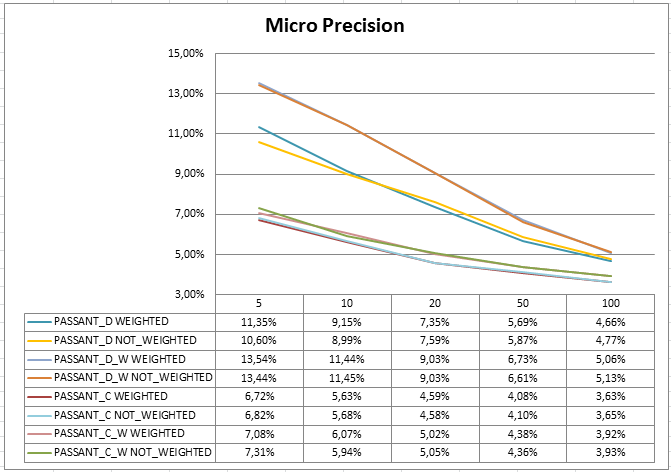
\includegraphics[width=\textwidth]{./images/graphs/micro_prec_Own}
	\caption{\emph{Config A - Micro precision}}
\end{figure}

\begin{figure}[H]
	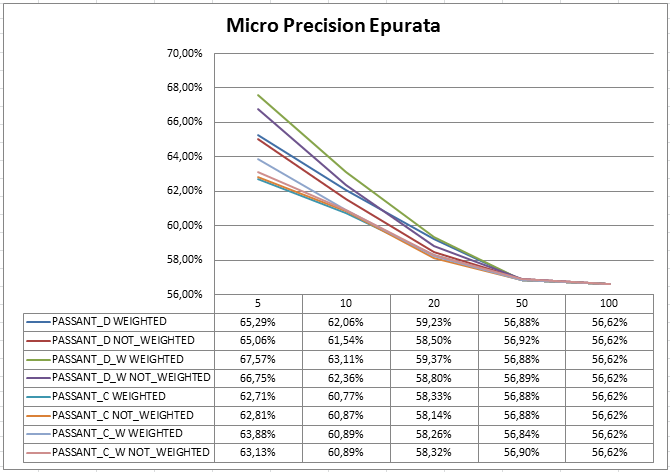
\includegraphics[width=\textwidth]{./images/graphs/micro_precT_Own}
	\caption{\emph{Config A - Micro precision epurata}}
\end{figure}

\subsection{Configurazione B}
Testando altri possibili valori da attribuire alle singole proprietà, si sono ottenuti questi risultati:
\begin{table}[H]
	\small
	\centering
	\begin{tabular}{l c}
		\textit{Properties} & \textit{Value} \\\hline
		editing & 0.2 \\
		music & 0.1 \\
		cinematography & 0.1 \\
		director & 0.7 \\
		distributor & 0.1 \\
		producer & 0.1 \\
		starring & 0.6 \\
		studio & 0.1 \\
		writer & 0.3 \\
		subject & 0.8 \\
	\end{tabular}
	\caption{\emph{Configurazione B}}
\end{table}

		% Table generated by 'ConfMusto'
\begin{table}[H]
	\centering
	\resizebox{.9\textwidth}{!}{%
		\begin{tabular}{ccccccc}
			{\bf K} & {\bf DISTANCE} & {\bf PROFILE} & {\bf MICRO\_PREC} & {\bf MICRO\_PREC\_T} & {\bf MICRO\_MRR} & {\bf MICRO\_MRR\_T} \\
			
			5 & PASSANT\_D\_W & NOT\_WEIGHTED &    12,10\% &    65,06\% &     7,34\% &    63,05\% \\
			
			5 & PASSANT\_D\_W &   WEIGHTED &    12,01\% &    66,49\% &     7,41\% &    64,17\% \\
			
			5 &  PASSANT\_D &   WEIGHTED &    11,35\% &    65,29\% &     6,65\% &    63,67\% \\
			
			5 &  PASSANT\_D & NOT\_WEIGHTED &    10,60\% &    65,06\% &     6,74\% &    63,03\% \\
			
			10 & PASSANT\_D\_W & NOT\_WEIGHTED &     9,98\% &    61,87\% &     7,34\% &    63,05\% \\
			
			10 & PASSANT\_D\_W &   WEIGHTED &     9,58\% &    62,62\% &     7,41\% &    64,17\% \\
			
			10 &  PASSANT\_D &   WEIGHTED &     9,15\% &    62,06\% &     6,65\% &    63,67\% \\
			
			10 &  PASSANT\_D & NOT\_WEIGHTED &     8,99\% &    61,54\% &     6,74\% &    63,03\% \\
			
			20 & PASSANT\_D\_W & NOT\_WEIGHTED &     8,15\% &    58,66\% &     7,34\% &    63,05\% \\
			
			20 & PASSANT\_D\_W &   WEIGHTED &     7,99\% &    59,36\% &     7,41\% &    64,17\% \\
			
			20 &  PASSANT\_D & NOT\_WEIGHTED &     7,59\% &    58,50\% &     6,74\% &    63,03\% \\
			
			20 &  PASSANT\_D &   WEIGHTED &     7,35\% &    59,23\% &     6,65\% &    63,67\% \\
			
			5 &  PASSANT\_C & NOT\_WEIGHTED &     6,82\% &    62,81\% &     4,69\% &    61,92\% \\
			
			5 &  PASSANT\_C &   WEIGHTED &     6,72\% &    62,71\% &     4,70\% &    62,42\% \\
			
			5 & PASSANT\_C\_W & NOT\_WEIGHTED &     6,49\% &    62,58\% &     4,67\% &    62,08\% \\
			
			5 & PASSANT\_C\_W &   WEIGHTED &     6,17\% &    63,03\% &     4,57\% &    62,24\% \\
			
			50 & PASSANT\_D\_W &   WEIGHTED &     6,14\% &    56,88\% &     7,41\% &    64,17\% \\
			
			50 & PASSANT\_D\_W & NOT\_WEIGHTED &     6,04\% &    56,88\% &     7,34\% &    63,05\% \\
			
			50 &  PASSANT\_D & NOT\_WEIGHTED &     5,87\% &    56,92\% &     6,74\% &    63,03\% \\
			
			50 &  PASSANT\_D &   WEIGHTED &     5,69\% &    56,88\% &     6,65\% &    63,67\% \\
			
			10 &  PASSANT\_C & NOT\_WEIGHTED &     5,68\% &    60,87\% &     4,69\% &    61,92\% \\
			
			10 &  PASSANT\_C &   WEIGHTED &     5,63\% &    60,77\% &     4,70\% &    62,42\% \\
			
			10 & PASSANT\_C\_W & NOT\_WEIGHTED &     5,50\% &    60,73\% &     4,67\% &    62,08\% \\
			
			10 & PASSANT\_C\_W &   WEIGHTED &     5,32\% &    60,38\% &     4,57\% &    62,24\% \\
			
			100 & PASSANT\_D\_W & NOT\_WEIGHTED &     4,96\% &    56,62\% &     7,34\% &    63,05\% \\
			
			100 & PASSANT\_D\_W &   WEIGHTED &     4,85\% &    56,62\% &     7,41\% &    64,17\% \\
			
			100 &  PASSANT\_D & NOT\_WEIGHTED &     4,77\% &    56,62\% &     6,74\% &    63,03\% \\
			
			20 & PASSANT\_C\_W & NOT\_WEIGHTED &     4,76\% &    58,03\% &     4,67\% &    62,08\% \\
			
			100 &  PASSANT\_D &   WEIGHTED &     4,66\% &    56,62\% &     6,65\% &    63,67\% \\
			
			20 & PASSANT\_C\_W &   WEIGHTED &     4,65\% &    58,23\% &     4,57\% &    62,24\% \\
			
			20 &  PASSANT\_C &   WEIGHTED &     4,59\% &    58,33\% &     4,70\% &    62,42\% \\
			
			20 &  PASSANT\_C & NOT\_WEIGHTED &     4,58\% &    58,14\% &     4,69\% &    61,92\% \\
			
			50 & PASSANT\_C\_W & NOT\_WEIGHTED &     4,19\% &    56,89\% &     4,67\% &    62,08\% \\
			
			50 & PASSANT\_C\_W &   WEIGHTED &     4,18\% &    56,88\% &     4,57\% &    62,24\% \\
			
			50 &  PASSANT\_C & NOT\_WEIGHTED &     4,10\% &    56,88\% &     4,69\% &    61,92\% \\
			
			50 &  PASSANT\_C &   WEIGHTED &     4,08\% &    56,88\% &     4,70\% &    62,42\% \\
			
			100 & PASSANT\_C\_W & NOT\_WEIGHTED &     3,80\% &    56,62\% &     4,67\% &    62,08\% \\
			
			100 & PASSANT\_C\_W &   WEIGHTED &     3,78\% &    56,62\% &     4,57\% &    62,24\% \\
			
			100 &  PASSANT\_C & NOT\_WEIGHTED &     3,65\% &    56,62\% &     4,69\% &    61,92\% \\
			
			100 &  PASSANT\_C &   WEIGHTED &     3,63\% &    56,62\% &     4,70\% &    62,42\% \\
			
		\end{tabular}  
	}
	\caption{\emph{Risultati configurazione B}}
\end{table}

\begin{table}[H]
	\centering
	\resizebox{.9\textwidth}{!}{%
		\begin{tabular}{ccccccc}
			{\bf K} & {\bf DISTANCE} & {\bf PROFILE} & {\bf MACRO\_PREC} & {\bf MACRO\_PREC\_T} & {\bf MACRO\_MRR} & {\bf MACRO\_MRR\_T} \\
			
			5 & PASSANT\_D\_W & NOT\_WEIGHTED &    12,10\% &    65,06\% &     7,36\% &    63,57\% \\
			
			5 & PASSANT\_D\_W &   WEIGHTED &    12,01\% &    66,49\% &     7,44\% &    64,57\% \\
			
			5 &  PASSANT\_D &   WEIGHTED &    11,35\% &    65,29\% &     6,68\% &    64,15\% \\
			
			5 &  PASSANT\_D & NOT\_WEIGHTED &    10,60\% &    65,06\% &     6,76\% &    63,58\% \\
			
			10 & PASSANT\_D\_W & NOT\_WEIGHTED &     9,98\% &    62,11\% &     7,36\% &    63,57\% \\
			
			10 & PASSANT\_D\_W &   WEIGHTED &     9,58\% &    62,81\% &     7,44\% &    64,57\% \\
			
			10 &  PASSANT\_D &   WEIGHTED &     9,15\% &    62,29\% &     6,68\% &    64,15\% \\
			
			10 &  PASSANT\_D & NOT\_WEIGHTED &     8,99\% &    61,80\% &     6,76\% &    63,58\% \\
			
			20 & PASSANT\_D\_W & NOT\_WEIGHTED &     8,15\% &    59,79\% &     7,36\% &    63,57\% \\
			
			20 & PASSANT\_D\_W &   WEIGHTED &     7,99\% &    60,30\% &     7,44\% &    64,57\% \\
			
			20 &  PASSANT\_D & NOT\_WEIGHTED &     7,59\% &    59,68\% &     6,76\% &    63,58\% \\
			
			20 &  PASSANT\_D &   WEIGHTED &     7,35\% &    60,21\% &     6,68\% &    64,15\% \\
			
			5 &  PASSANT\_C & NOT\_WEIGHTED &     6,82\% &    62,81\% &     4,71\% &    62,63\% \\
			
			5 &  PASSANT\_C &   WEIGHTED &     6,72\% &    62,71\% &     4,73\% &    63,06\% \\
			
			5 & PASSANT\_C\_W & NOT\_WEIGHTED &     6,49\% &    62,58\% &     4,68\% &    62,79\% \\
			
			5 & PASSANT\_C\_W &   WEIGHTED &     6,17\% &    63,03\% &     4,60\% &    62,91\% \\
			
			50 & PASSANT\_D\_W &   WEIGHTED &     6,14\% &    59,11\% &     7,44\% &    64,57\% \\
			
			50 & PASSANT\_D\_W & NOT\_WEIGHTED &     6,04\% &    59,11\% &     7,36\% &    63,57\% \\
			
			50 &  PASSANT\_D & NOT\_WEIGHTED &     5,87\% &    59,12\% &     6,76\% &    63,58\% \\
			
			50 &  PASSANT\_D &   WEIGHTED &     5,69\% &    59,11\% &     6,68\% &    64,15\% \\
			
			10 &  PASSANT\_C & NOT\_WEIGHTED &     5,68\% &    61,18\% &     4,71\% &    62,63\% \\
			
			10 &  PASSANT\_C &   WEIGHTED &     5,63\% &    61,08\% &     4,73\% &    63,06\% \\
			
			10 & PASSANT\_C\_W & NOT\_WEIGHTED &     5,50\% &    61,05\% &     4,68\% &    62,79\% \\
			
			10 & PASSANT\_C\_W &   WEIGHTED &     5,32\% &    60,72\% &     4,60\% &    62,91\% \\
			
			100 & PASSANT\_D\_W & NOT\_WEIGHTED &     4,96\% &    59,08\% &     7,36\% &    63,57\% \\
			
			100 & PASSANT\_D\_W &   WEIGHTED &     4,85\% &    59,08\% &     7,44\% &    64,57\% \\
			
			100 &  PASSANT\_D & NOT\_WEIGHTED &     4,77\% &    59,08\% &     6,76\% &    63,58\% \\
			
			20 & PASSANT\_C\_W & NOT\_WEIGHTED &     4,76\% &    59,33\% &     4,68\% &    62,79\% \\
			
			100 &  PASSANT\_D &   WEIGHTED &     4,66\% &    59,08\% &     6,68\% &    64,15\% \\
			
			20 & PASSANT\_C\_W &   WEIGHTED &     4,65\% &    59,47\% &     4,60\% &    62,91\% \\
			
			20 &  PASSANT\_C &   WEIGHTED &     4,59\% &    59,55\% &     4,73\% &    63,06\% \\
			
			20 &  PASSANT\_C & NOT\_WEIGHTED &     4,58\% &    59,41\% &     4,71\% &    62,63\% \\
			
			50 & PASSANT\_C\_W & NOT\_WEIGHTED &     4,19\% &    59,11\% &     4,68\% &    62,79\% \\
			
			50 & PASSANT\_C\_W &   WEIGHTED &     4,18\% &    59,11\% &     4,60\% &    62,91\% \\
			
			50 &  PASSANT\_C & NOT\_WEIGHTED &     4,10\% &    59,11\% &     4,71\% &    62,63\% \\
			
			50 &  PASSANT\_C &   WEIGHTED &     4,08\% &    59,11\% &     4,73\% &    63,06\% \\
			
			100 & PASSANT\_C\_W & NOT\_WEIGHTED &     3,80\% &    59,08\% &     4,68\% &    62,79\% \\
			
			100 & PASSANT\_C\_W &   WEIGHTED &     3,78\% &    59,08\% &     4,60\% &    62,91\% \\
			
			100 &  PASSANT\_C & NOT\_WEIGHTED &     3,65\% &    59,08\% &     4,71\% &    62,63\% \\
			
			100 &  PASSANT\_C &   WEIGHTED &     3,63\% &    59,08\% &     4,73\% &    63,06\% \\
			
		\end{tabular}  
}
	\caption{\emph{Risultati configurazione B}}
\end{table}

Analizzando anche in questo caso i valori ottenuti nelle due metriche prese in considerazione anche nella configurazione precedente, otteniamo i seguenti grafici:
\begin{figure}[H]
	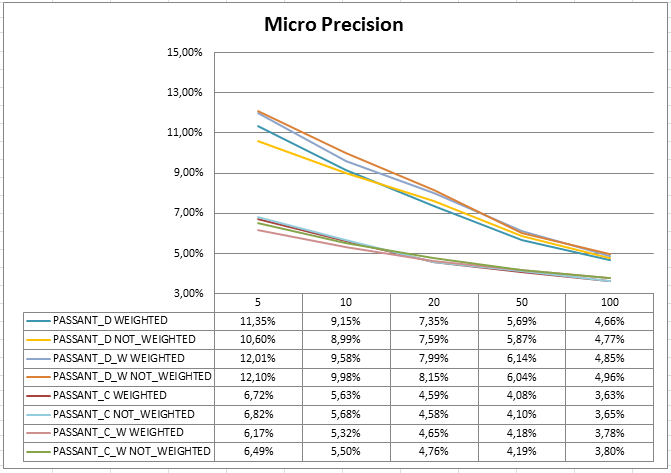
\includegraphics[width=.9\textwidth]{./images/graphs/micro_prec_Musto}
	\caption{\emph{Config B - Micro precision}}
\end{figure}

\begin{figure}[H]
	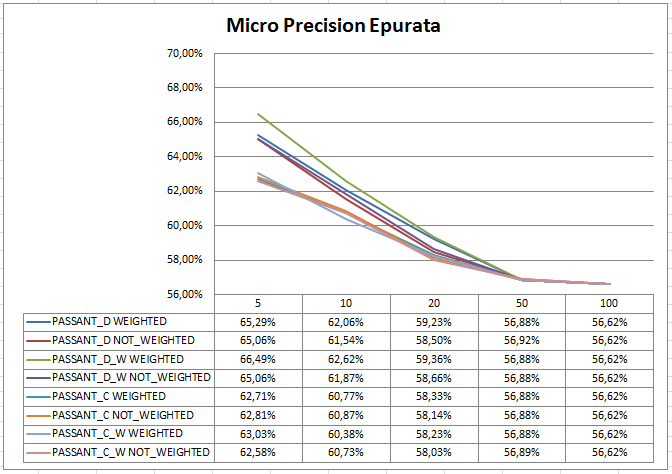
\includegraphics[width=.9\textwidth]{./images/graphs/micro_precT_Musto}
	\caption{\emph{Config B - Micro precision epurata}}
\end{figure}
Cosi come accadeva in precedenza, tipologia che permette di ottenere le prestazioni migliori è sempre a distanza diretta e pesata di Passant in entrambe le varianti di profilazione.

\subsection{Configurazione C}
La terza configurazione presa in esame, sarà settata in modo tale da prendere in considerazione solo le proprietà che si potrebbero reputare importanti ai fini di una ipotetica raccomandazione, annullando tutte quelle proprietà che si reputano inutili e che potrebbero influenzare negativamente la raccomandazione inserendo eventuale rumore nei dati. Di seguito il settaggio e i risultati della raccomandazione:
\begin{table}[H]
	\small
	\centering
	\begin{tabular}{l l}
		\textit{Properties} & \textit{Value} \\\hline
		editing & 0 \\
		music & 0.31 \\
		cinematography & 0\\
		director & 0.83\\
		distributor & 0\\
		producer & 0 \\
		starring & 0.50\\
		studio & 0\\
		writer & 0\\
		subject & 0.23\\
	\end{tabular}
	\caption{\emph{Configurazione C}}
\end{table}

% Table generated by 'MaxRaggiunto'
\begin{table}[H]
	\centering
	\resizebox{.9\textwidth}{!}{%
\begin{tabular}{ccccccc}
	
	{\bf K} & {\bf DISTANCE} & {\bf PROFILE} & {\bf MICRO\_PREC} & {\bf MICRO\_PREC\_T} & {\bf MICRO\_MRR} & {\bf MICRO\_MRR\_T} \\
	
	5 & PASSANT\_D\_W &   WEIGHTED &    14,55\% &    68,97\% &     8,89\% &    65,97\% \\
	
	5 & PASSANT\_D\_W & NOT\_WEIGHTED &    13,93\% &    67,73\% &     8,60\% &    64,67\% \\
	
	10 & PASSANT\_D\_W &   WEIGHTED &    12,51\% &    63,51\% &     8,89\% &    65,97\% \\
	
	10 & PASSANT\_D\_W & NOT\_WEIGHTED &    12,09\% &    62,81\% &     8,60\% &    64,67\% \\
	
	5 &  PASSANT\_D &   WEIGHTED &    11,35\% &    65,29\% &     6,65\% &    63,67\% \\
	
	5 &  PASSANT\_D & NOT\_WEIGHTED &    10,60\% &    65,06\% &     6,74\% &    63,03\% \\
	
	5 & PASSANT\_C\_W &   WEIGHTED &    10,15\% &    65,12\% &     6,48\% &    63,22\% \\
	
	20 & PASSANT\_D\_W & NOT\_WEIGHTED &    10,06\% &    59,06\% &     8,60\% &    64,67\% \\
	
	20 & PASSANT\_D\_W &   WEIGHTED &    10,02\% &    59,72\% &     8,89\% &    65,97\% \\
	
	5 & PASSANT\_C\_W & NOT\_WEIGHTED &     9,85\% &    64,50\% &     6,13\% &    62,69\% \\
	
	10 &  PASSANT\_D &   WEIGHTED &     9,15\% &    62,06\% &     6,65\% &    63,67\% \\
	
	10 &  PASSANT\_D & NOT\_WEIGHTED &     8,99\% &    61,54\% &     6,74\% &    63,03\% \\
	
	10 & PASSANT\_C\_W &   WEIGHTED &     7,65\% &    61,80\% &     6,48\% &    63,22\% \\
	
	20 &  PASSANT\_D & NOT\_WEIGHTED &     7,59\% &    58,50\% &     6,74\% &    63,03\% \\
	
	20 &  PASSANT\_D &   WEIGHTED &     7,35\% &    59,23\% &     6,65\% &    63,67\% \\
	
	10 & PASSANT\_C\_W & NOT\_WEIGHTED &     7,29\% &    61,40\% &     6,13\% &    62,69\% \\
	
	50 & PASSANT\_D\_W &   WEIGHTED &     7,20\% &    56,94\% &     8,89\% &    65,97\% \\
	
	50 & PASSANT\_D\_W & NOT\_WEIGHTED &     7,05\% &    56,92\% &     8,60\% &    64,67\% \\
	
	5 &  PASSANT\_C & NOT\_WEIGHTED &     6,82\% &    62,81\% &     4,69\% &    61,92\% \\
	
	5 &  PASSANT\_C &   WEIGHTED &     6,72\% &    62,71\% &     4,70\% &    62,42\% \\
	
	20 & PASSANT\_C\_W &   WEIGHTED &     5,98\% &    58,66\% &     6,48\% &    63,22\% \\
	
	50 &  PASSANT\_D & NOT\_WEIGHTED &     5,87\% &    56,92\% &     6,74\% &    63,03\% \\
	
	50 &  PASSANT\_D &   WEIGHTED &     5,69\% &    56,88\% &     6,65\% &    63,67\% \\
	
	10 &  PASSANT\_C & NOT\_WEIGHTED &     5,68\% &    60,87\% &     4,69\% &    61,92\% \\
	
	20 & PASSANT\_C\_W & NOT\_WEIGHTED &     5,65\% &    58,48\% &     6,13\% &    62,69\% \\
	
	10 &  PASSANT\_C &   WEIGHTED &     5,63\% &    60,77\% &     4,70\% &    62,42\% \\
	
	100 & PASSANT\_D\_W &   WEIGHTED &     5,31\% &    56,62\% &     8,89\% &    65,97\% \\
	
	100 & PASSANT\_D\_W & NOT\_WEIGHTED &     5,30\% &    56,62\% &     8,60\% &    64,67\% \\
	
	50 & PASSANT\_C\_W &   WEIGHTED &     5,09\% &    56,87\% &     6,48\% &    63,22\% \\
	
	50 & PASSANT\_C\_W & NOT\_WEIGHTED &     4,92\% &    56,89\% &     6,13\% &    62,69\% \\
	
	100 &  PASSANT\_D & NOT\_WEIGHTED &     4,77\% &    56,62\% &     6,74\% &    63,03\% \\
	
	100 &  PASSANT\_D &   WEIGHTED &     4,66\% &    56,62\% &     6,65\% &    63,67\% \\
	
	20 &  PASSANT\_C &   WEIGHTED &     4,59\% &    58,33\% &     4,70\% &    62,42\% \\
	
	20 &  PASSANT\_C & NOT\_WEIGHTED &     4,58\% &    58,14\% &     4,69\% &    61,92\% \\
	
	100 & PASSANT\_C\_W &   WEIGHTED &     4,25\% &    56,62\% &     6,48\% &    63,22\% \\
	
	100 & PASSANT\_C\_W & NOT\_WEIGHTED &     4,15\% &    56,62\% &     6,13\% &    62,69\% \\
	
	50 &  PASSANT\_C & NOT\_WEIGHTED &     4,10\% &    56,88\% &     4,69\% &    61,92\% \\
	
	50 &  PASSANT\_C &   WEIGHTED &     4,08\% &    56,88\% &     4,70\% &    62,42\% \\
	
	100 &  PASSANT\_C & NOT\_WEIGHTED &     3,65\% &    56,62\% &     4,69\% &    61,92\% \\
	
	100 &  PASSANT\_C &   WEIGHTED &     3,63\% &    56,62\% &     4,70\% &    62,42\% \\
	
	\end{tabular}  	
}
	\caption{\emph{Risultati configurazione C}}
\end{table}

\begin{table}[H]
	\centering
	\resizebox{.9\textwidth}{!}{%
		\begin{tabular}{ccccccc}
			
			{\bf K} & {\bf DISTANCE} & {\bf PROFILE} & {\bf MACRO\_PREC} & {\bf MACRO\_PREC\_T} & {\bf MACRO\_MRR} & {\bf MACRO\_MRR\_T} \\
			
			5 & PASSANT\_D\_W &   WEIGHTED &    14,55\% &    68,97\% &     8,94\% &    66,24\% \\
			
			5 & PASSANT\_D\_W & NOT\_WEIGHTED &    13,93\% &    67,73\% &     8,63\% &    65,05\% \\
			
			10 & PASSANT\_D\_W &   WEIGHTED &    12,51\% &    63,64\% &     8,94\% &    66,24\% \\
			
			10 & PASSANT\_D\_W & NOT\_WEIGHTED &    12,09\% &    62,99\% &     8,63\% &    65,05\% \\
			
			5 &  PASSANT\_D &   WEIGHTED &    11,35\% &    65,29\% &     6,68\% &    64,15\% \\
			
			5 &  PASSANT\_D & NOT\_WEIGHTED &    10,60\% &    65,06\% &     6,76\% &    63,58\% \\
			
			5 & PASSANT\_C\_W &   WEIGHTED &    10,15\% &    65,12\% &     6,51\% &    63,75\% \\
			
			20 & PASSANT\_D\_W & NOT\_WEIGHTED &    10,06\% &    60,08\% &     8,63\% &    65,05\% \\
			
			20 & PASSANT\_D\_W &   WEIGHTED &    10,02\% &    60,57\% &     8,94\% &    66,24\% \\
			
			5 & PASSANT\_C\_W & NOT\_WEIGHTED &     9,85\% &    64,50\% &     6,15\% &    63,27\% \\
			
			10 &  PASSANT\_D &   WEIGHTED &     9,15\% &    62,29\% &     6,68\% &    64,15\% \\
			
			10 &  PASSANT\_D & NOT\_WEIGHTED &     8,99\% &    61,80\% &     6,76\% &    63,58\% \\
			
			10 & PASSANT\_C\_W &   WEIGHTED &     7,65\% &    62,05\% &     6,51\% &    63,75\% \\
			
			20 &  PASSANT\_D & NOT\_WEIGHTED &     7,59\% &    59,68\% &     6,76\% &    63,58\% \\
			
			20 &  PASSANT\_D &   WEIGHTED &     7,35\% &    60,21\% &     6,68\% &    64,15\% \\
			
			10 & PASSANT\_C\_W & NOT\_WEIGHTED &     7,29\% &    61,67\% &     6,15\% &    63,27\% \\
			
			50 & PASSANT\_D\_W &   WEIGHTED &     7,20\% &    59,13\% &     8,94\% &    66,24\% \\
			
			50 & PASSANT\_D\_W & NOT\_WEIGHTED &     7,05\% &    59,12\% &     8,63\% &    65,05\% \\
			
			5 &  PASSANT\_C & NOT\_WEIGHTED &     6,82\% &    62,81\% &     4,71\% &    62,63\% \\
			
			5 &  PASSANT\_C &   WEIGHTED &     6,72\% &    62,71\% &     4,73\% &    63,06\% \\
			
			20 & PASSANT\_C\_W &   WEIGHTED &     5,98\% &    59,79\% &     6,51\% &    63,75\% \\
			
			50 &  PASSANT\_D & NOT\_WEIGHTED &     5,87\% &    59,12\% &     6,76\% &    63,58\% \\
			
			50 &  PASSANT\_D &   WEIGHTED &     5,69\% &    59,11\% &     6,68\% &    64,15\% \\
			
			10 &  PASSANT\_C & NOT\_WEIGHTED &     5,68\% &    61,18\% &     4,71\% &    62,63\% \\
			
			20 & PASSANT\_C\_W & NOT\_WEIGHTED &     5,65\% &    59,66\% &     6,15\% &    63,27\% \\
			
			10 &  PASSANT\_C &   WEIGHTED &     5,63\% &    61,08\% &     4,73\% &    63,06\% \\
			
			100 & PASSANT\_D\_W &   WEIGHTED &     5,31\% &    59,08\% &     8,94\% &    66,24\% \\
			
			100 & PASSANT\_D\_W & NOT\_WEIGHTED &     5,30\% &    59,08\% &     8,63\% &    65,05\% \\
			
			50 & PASSANT\_C\_W &   WEIGHTED &     5,09\% &    59,10\% &     6,51\% &    63,75\% \\
			
			50 & PASSANT\_C\_W & NOT\_WEIGHTED &     4,92\% &    59,11\% &     6,15\% &    63,27\% \\
			
			100 &  PASSANT\_D & NOT\_WEIGHTED &     4,77\% &    59,08\% &     6,76\% &    63,58\% \\
			
			100 &  PASSANT\_D &   WEIGHTED &     4,66\% &    59,08\% &     6,68\% &    64,15\% \\
			
			20 &  PASSANT\_C &   WEIGHTED &     4,59\% &    59,55\% &     4,73\% &    63,06\% \\
			
			20 &  PASSANT\_C & NOT\_WEIGHTED &     4,58\% &    59,41\% &     4,71\% &    62,63\% \\
			
			100 & PASSANT\_C\_W &   WEIGHTED &     4,25\% &    59,08\% &     6,51\% &    63,75\% \\
			
			100 & PASSANT\_C\_W & NOT\_WEIGHTED &     4,15\% &    59,08\% &     6,15\% &    63,27\% \\
			
			50 &  PASSANT\_C & NOT\_WEIGHTED &     4,10\% &    59,11\% &     4,71\% &    62,63\% \\
			
			50 &  PASSANT\_C &   WEIGHTED &     4,08\% &    59,11\% &     4,73\% &    63,06\% \\
			
			100 &  PASSANT\_C & NOT\_WEIGHTED &     3,65\% &    59,08\% &     4,71\% &    62,63\% \\
			
			100 &  PASSANT\_C &   WEIGHTED &     3,63\% &    59,08\% &     4,73\% &    63,06\% \\
			
		\end{tabular}  		 	
	}
	\caption{\emph{Risultati configurazione C}}
\end{table}

Come nei due casi precedenti, verranno analizzati sia la microprecision che la microprecision epurata:
\begin{figure}[H]
	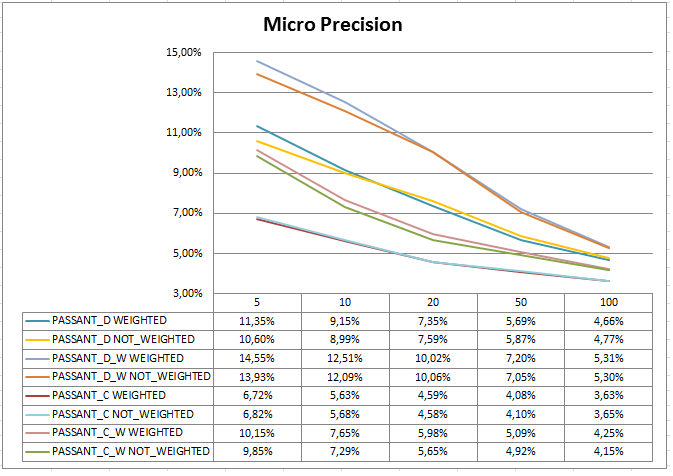
\includegraphics[width=.9\textwidth]{./images/graphs/micro_prec_Best}
	\caption{\emph{Config C - Micro precision}}
\end{figure}

\begin{figure}[H]
	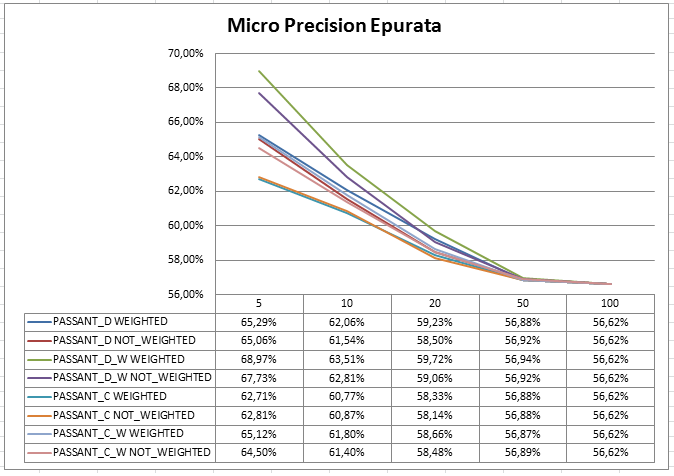
\includegraphics[width=.9\textwidth]{./images/graphs/micro_precT_Best}
	\caption{\emph{Config C - Micro precision epurata}}
\end{figure}

Come si evince da questi grafici, anche in questo caso, i risultati migliori sono quelli espressi sempre dalla distanza diretta e pesata di passant in entrambe le versioni di profilazione. 

\subsection{Considerazioni}
Mettendo a confronto i risultati migliori ottenuti dalle diverse configurazioni, si evince che la configurazione che ha fatto ottenere i risultati migliori sia in termini di precisione, che in termini di precisione epurata, sia stata l'ultima configurazione presa in esame.

\subsubsection{Microprecision}
In particolar modo, per quanto riguarda la microprecision, ecco un grafico riassuntivo che mette a confronto i risultati migliori ottenuti dalle tre configurazioni:

\begin{figure}
\begin{tikzpicture}
\begin{axis}[
xmin=0,     
xmax=100,    
ymin=4,     
ymax=16,
ylabel=\%,
xlabel= $k$,
/pgfplots/xtick={5,10,20,50,100}, 
legend style={
	%font=\tiny,
	%pos=outer north east,
	%line width=.1pt,
	%mark size=.6pt
},
width=.9\textwidth,
height=.8\textwidth,
grid=both, 
axis background/.style={fill=white}]
\addplot[color=silver,thick] coordinates {
	(5,13.54)
	(10,11.44)
	(20,9.03)
	(50,6.73)
	(100,5.06)
	
};
\addlegendentry{CONFIG A} % conf A = nostra

\addplot[color=bronze,thick] coordinates {
	(5,12.10)
	(10,9.98)
	(20,8.15)
	(50,6.04)
	(100,4.85)
};
\addlegendentry{CONFIG B} % conf B = musto

\addplot[color=gold,thick] coordinates {
	(5,14.55)
	(10,12.51)
	(20,10.02)
	(50,7.20)
	(100,5.31)
};
\addlegendentry{CONFIG C} % conf C = max raggiunto

\addplot[color=black,thick] coordinates {
	(5,11.35)
	(10,9.15)
	(20,7.35)
	(50,5.69)
	(100,4.66)
};
\addlegendentry{BASELINE}
\end{axis}
\end{tikzpicture}
\caption{\emph{Confronto delle migliori precision}}
\end{figure}
Come si può constatare, prendendo in considerazione le pesature non omogenee tra gli archi, si è riusciti ad ottenere un miglioramento percentuale della precisione nel sistema di raccomandazione pari a :

\begin{itemize}
	\item +3.2 \% per $k = 5 $
	\item +3.36 \% per $k = 10 $
	\item +2.67 \% per $k = 20 $
	\item +1.51 \% per $k = 50 $
	\item +0.65 \% per $k = 100 $				
\end{itemize} 

\subsubsection{Microprecision Epurata}
Prendendo in considerazione invece le microprecision epurate, otteniamo i seguenti risultati:
\begin{figure}
	\begin{tikzpicture}
	\begin{axis}[
	xmin=0,     
	xmax=100,    
	ymin=56,
	ymax=70,     
	ylabel=\%,
	xlabel= $k$,
	/pgfplots/xtick={5,10,20,50,100}, 
	legend style={
		%font=\tiny,
		%pos=outer north east,
		%line width=.1pt,
		%mark size=.6pt
	},
	width=.9\textwidth,
	height=.8\textwidth,
	grid=both, 
	axis background/.style={fill=white}]
	\addplot[color=silver,thick] coordinates {
		(5,67.57)
		(10,63.11)
		(20,59.37)
		(50,56.88)
		(100,56.62)
		
	};
	\addlegendentry{CONFIG A} % conf A = nostra
	
	\addplot[color=bronze,thick] coordinates {
		(5,66.49)
		(10,62.62)
		(20,59.36)
		(50,56.88)
		(100,56.62)
	};
	\addlegendentry{CONFIG B} % conf B = musto
	
	\addplot[color=gold,thick] coordinates {
		(5,68.97)
		(10,63.51)
		(20,59.72)
		(50,56.94)
		(100,56.62)
	};
	\addlegendentry{CONFIG C} % conf C = max raggiunto
	
	\addplot[color=black,thick] coordinates {
		(5,65.29)
		(10,62.06)
		(20,59.23)
		(50,56.88)
		(100,56.62)
	};
	\addlegendentry{BASELINE}
	\end{axis}
	\end{tikzpicture}
	\caption{\emph{Confronto delle migliori precision epurate}}
\end{figure}

Anche in questo caso si può constatare che, prendendo in considerazione le pesature non omogenee tra gli archi, si è riusciti ad ottenere un miglioramento percentuale della precisione nel sistema di raccomandazione pari a :

\begin{itemize}
	\item +3.68 \% per $k = 5 $
	\item +1.45 \% per $k = 10 $
	\item +0.49 \% per $k = 20 $
	\item +0.06 \% per $k = 50 $
	\item 0\footnote{Non si è riuscito ad ottenere nessun miglioramento a causa della quantità di film profilati dagli utenti (< 100) } \% per $k = 100 $				
\end{itemize} 
